\documentclass[a4paper, 14pt]{extarticle}

\usepackage{../../latexDependencies/misc/preamble2}

\geometry{a4paper}

% Название дисциплины
\newcommand{\subject}{Теория вероятности и математическая статистика} 

% Тип работы
% lab - для лабораторной работы 
% hw  - для домашней     работы
\newcommand{\task}{lab} 

% Номер работы
\newcommand{\taskNumber}{3} 

% Название работы
\newcommand{\taskNameOne}{Моделирование выборки из абсолютно непрерывного } 
\newcommand{\taskNameTwo}{закона распределения методом обратных функций.} 

% Имя студента
\newcommand{\studentName}{Очкин Н.В.}

% Имя преподававателя
\newcommand{\teacherName}{Облакова Т.В.}

% Группа
\newcommand{\group}{ФН11-52Б}

% Вариант
\newcommand{\variant}{9}

\begin{document}

\graphicspath{ {../../latexDependencies/images} } 
\normalsize

\newcommand{\printTask}{%
    \ifthenelse{\equal{\task}{lab}}{%
        лабораторной%
    }{%
        \ifthenelse{\equal{\task}{hw}}{%
            домашней%
        }{%
            Неизвестный тип задания%
        }%
    }%
}

\begin{titlepage}

    \begin{center}
        {\footnotesize \itshape Федеральное государственное бюджетное 
                       образовательное учреждение высшего образования}
    \end{center}

    \begin{minipage}[c]{0.1\textwidth}
        
\includegraphics[width=1.1\textwidth]{iconBMSTU}
    \end{minipage}
    \hfill
    \begin{minipage}[c]{0.9\textwidth}
        \centering
        \itshape
        \bfseries
        \small
        \guillemotleft Московский государственный технический университет \\
        имени Н.Э. Баумана\guillemotright \\
        (национальный исследовательский университет) \\
        (МГТУ им. Н.Э. Баумана) 
    \end{minipage}

    \vspace{0.5cm}
    \noindent\rule{\textwidth}{2pt} \\

    \noindent\uline{\textbf{ФАКУЛЬТЕТ} ФУНДАМЕНТАЛЬНЫЕ НАУКИ} \\
    \vspace{-5pt} \\
    \noindent\uline{\textbf{КАФЕДРА} ВЫЧИСЛИТЕЛЬНАЯ МАТЕМАТИКА И МАТЕМАТИЧЕСКАЯ} \\
    \vspace{-5pt} \\
    \noindent\uline{ФИЗИКА (ФН11)} \\
    \vspace{-5pt} \\
    \noindent\uline{\textbf{НАПРАВЛЕНИЕ ПОДГОТОВКИ} МАТЕМАТИКА И КОМПЬЮТЕРНЫЕ} \\
    \vspace{-5pt} \\
    \noindent\uline{НАУКИ (02.03.01)} \\

    \begin{center}
        \bfseries
        \textsc{О т ч е т} \\[10pt]
        по \printTask {} работе \textnumero {} \taskNumber
    \end{center}

    \vspace{10pt}

    \hspace{10pt} 
    \noindent \textbf{Название \printTask {} работы:} \par
    \vspace{5pt}
    \hspace{10pt} 
    \noindent \textbf{\uline{\taskNameOne}} \vspace{5pt} \\
    \null\hspace{31pt} 
    \textbf{\uline{\taskNameTwo}} \vspace{5pt} 

    \vspace{10pt}

    \begin{center}
        \bfseries
        Вариант \textnumero {} \variant
    \end{center}

    \vspace{20pt}

    \hspace{10pt} 
    \noindent \textbf{Дисциплина:} \par
    \vspace{10pt}
    \hspace{10pt} 
    \noindent {\large \subject}

    \vspace{10pt}

    \begin{flushright}
        \renewcommand{\arraystretch}{3}
        \begin{tabular}{r r r}
            \multicolumn{1}{l}{Студент группы \uline{\group}} & 
            $\quad \underset{\text{(Подпись, дата)}}{\underline{\hspace{3cm}}} \quad$ & 
            \multicolumn{1}{c}{$\underset{\text{(И.О. Фамилия)}}{\uline{\textbf{\studentName}}}$} \\

            \multicolumn{1}{l}{Преподаватель} & 
            $\quad \underset{\text{(Подпись, дата)}}{\underline{\hspace{3cm}}} \quad$ & 
            \multicolumn{1}{c}{$\underset{\text{(И.О. Фамилия)}}{\uline{\textbf{\teacherName}}}$} \\
        \end{tabular}
    \end{flushright}

    \vfill

    \begin{center}
        \small
        Москва, 2024
    \end{center}
\end{titlepage}


\newgeometry{left=25mm, right=25mm, top=20mm, bottom=20mm}

\graphicspath{ {../../latexDependencies/images/LW3} }

% Customize section, subsection, subsubsection and paragraph styles
\titleformat{\section}
  {\normalfont\large\bfseries}{\thesection}{1em}{}

\titleformat{\subsection}
  {\normalfont\normalsize\bfseries}{\thesubsection}{1em}{}

\titleformat{\subsubsection}
  {\normalfont\small\bfseries}{\thesubsubsection}{1em}{}

\titleformat{\paragraph}
  {\small\small\bfseries}{\theparagraph}{1em}{}

\thispagestyle{empty}

\null\newpage

\setcounter{tocdepth}{5}
\setcounter{secnumdepth}{5}

\pagenumbering{roman}

\tableofcontents
\newpage

\pagenumbering{arabic}
\setcounter{page}{1}

\setstretch{1}
\linespread{1.1}

\setlength{\parindent}{0pt}

\fontsize{12pt}{16pt}\selectfont

% --------------------------------------START--------------------------------------

\section{Задание}\vspace{-20pt}\rule{\linewidth}{0.1mm}

\begin{enumerate}
  \item Для данного $n$ методом обратных функций смоделируйте выборку 
  из закона распределения с заданной плотностью  $p(x)$.
  \item Для полученной выборки найдите гистограмму относительных частот. 
  Постройте на одном рисунке графики теоретической плотности $p(x)$ и 
  гистограмму относительных частот.
  \item Вычислите выборочное среднее и выборочную дисперсию и сравните с 
  истинными значениями этих характеристик.
  \item Используя неравенство \high{Dvoretzky-Kiefer-Wolfowitz}, 
  постройте 90\% доверительный интервал для функции распределения $F(x)$.
\end{enumerate}

Приведите графическую иллюстрацию

\section{Исходные данные}\vspace{-20pt}\rule{\linewidth}{0.1mm}

\begin{equation*}
  \text{Вариант: }9 \qquad n: 120
\end{equation*}
\begin{equation}
  \scalebox{1.25}{$p(x) = \cfrac{1}{\sqrt{0.4 \pi}x} e^{-(\ln{x} - 2)^2 / 0.4}, \quad x > 0$}
\end{equation}

\section{Решение}

\subsection{Часть 1}\vspace{-20pt}\rule{\linewidth}{0.1mm}
Для данного $n$ методом обратных функций смоделируйте выборку 
из закона распределения с заданной плотностью  $p(x)$.\\

\subsubsection{Функция распределения}\vspace{-20pt}\rule{\linewidth}{0.1mm}

Найдем функцию распределения:
\begin{equation}
    F_X(x) = \int_{-\infty}^{x} f_X(t) dt, \quad \text{где}
\end{equation}
$f_X(x)$ - плотность распределения.\\

Подставим (1) в (2):
\begin{gather*}
    F_X(x) = 
    \int_{0}^{x} \cfrac{1}{\sqrt{0.4 \pi}y} e^{-(\ln{y} - 2)^2 / 0.4} dy = \\[1em]
    = \left[\hspace{5pt}
    \begin{aligned}
        & t          = \frac{\ln(y)-2}{\sqrt{0.4}}          \qquad & dt &   = \frac{1}{y \sqrt{0.4}} dy   \\
        & \ln(y) - 2 = t \sqrt{0.4}                         \qquad & dy &   = y \sqrt{0.4} dt             \\
        & \ln(y)     = t \sqrt{0.4} + 2                     \qquad & x: & \hspace{5pt} t = \frac{\ln(x)-2}{\sqrt{0.4}} \\
        & y          = \exp \left[ t \sqrt{0.4} + 2 \right] \qquad & 0: & \hspace{5pt} t = -\infty                     \\ 
    \end{aligned}\,
    \hspace{5pt}\right] = \\[1em]
    = \cfrac{1}{\sqrt{0.4 \pi}} \int_{-\infty}^{\frac{\ln(x)-2}{\sqrt{0.4}}} e^{\left[ -t \sqrt{0.4} -2 \right]} 
    \cdot e^{-t^2} \cdot e^{\left[ t \sqrt{0.4} +2 \right]} \cdot \sqrt{0.4} dt = \\[1em]
    = \cfrac{1}{\sqrt{\pi}} \int_{-\infty}^{\frac{\ln(x)-2}{\sqrt{0.4}}} e^{-t^2} dt 
    = \frac{1}{\sqrt{\pi}} \left( \int_{-\infty}^{0} e^{-t^2} dt + \int_{0}^{\frac{\ln(x)-2}{\sqrt{0.4}}} e^{-t^2} dt \right) = \\[1em]
    = \frac{1}{\sqrt{\pi}} \left( \frac{\pi}{2} \text{erf} (t) \bigg|^0_{-\infty} + \frac{\sqrt{\pi}}{2} \cdot 
    \text{erf} \left( \cfrac{\ln(x)-2}{\sqrt{0.4}} \right) \right) \oeq
\end{gather*}\\
\vspace{10pt}
\hdashrule[0.5ex][c]{1\textwidth}{0.4pt}{3mm}
\begin{center}
    где erf(x) - \textbf{функция ошибок} (также называемая функция ошибок Гаусса).\\
\end{center}

\begin{minipage}[c]{0.5\textwidth}
    \begin{equation*}
        \scalebox{1.25}{$\text{erf} (x) = \cfrac{2}{\sqrt{\pi}} \int_{0}^{x} e^{-t^2} dt$}
    \end{equation*}
\end{minipage}
\hfill
\begin{minipage}[c]{0.5\textwidth}
    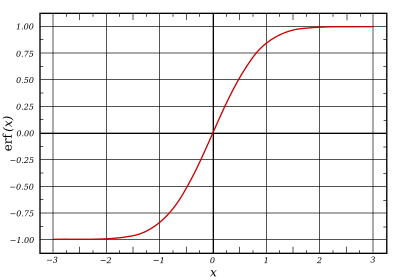
\includegraphics[width=1\textwidth]{Error_Function.svg}
\end{minipage}\\

{\footnotesize \textbf{Примечание:} из графика видно, что erf(0) = 0, erf($-\infty$) = -1}

\hdashrule[0.5ex][c]{1\textwidth}{0.4pt}{3mm}

\begin{gather*}
    \oeq \hspace{3pt} \frac{1}{\pi} \left( \frac{\pi}{2} \left( 0 - \left( -1 \right) \right) + 
    \frac{\pi}{2} \cdot \text{erf} \left( \cfrac{\ln(x)-2}{\sqrt{0.4}} \right) \right) = \\[1em]
    = \frac{1}{\pi} \left( \frac{\pi}{2} + \frac{\pi}{2} \cdot \text{erf} \left( 
    \cfrac{\ln(x) - 2}{\sqrt{0.4}} \right) \right) = \\[1em]
    = \cfrac{1}{2} + \cfrac{1}{2} \text{erf} \left( \cfrac{\ln(x) - 2}{\sqrt{0.4}} \right)
\end{gather*}\\
\vspace{-10pt}
В конечном итоге, функция распределения имеет вид\\[1em]
\begin{equation}
    F_X(x) = \cfrac{1}{2} + \cfrac{1}{2} \text{erf} \left( \cfrac{\ln(x) - 2}{\sqrt{0.4}} \right)
\end{equation}

\subsubsection{Обратная функция}\vspace{-20pt}\rule{\linewidth}{0.1mm}

Так как для нахождения обратной функции распределения требуется найти обратную 
функцию ошибок, что аналитически сделать сложно, воспользуемся численными методами.

\paragraph{Метод Ньютона}\vspace{-20pt}\rule{\linewidth}{0.1mm}

Для нахождения обратной функции воспользуемся методом касательных (Ньютона). \\
Рабочая формула
\begin{equation*}
  x_{n+1} = x_n - \cfrac{f(x_n)}{f'(x_n)}
\end{equation*}
Вообще говоря, метод используется для нахождения корня заданной функции. Так что 
для нахождения обратной функции $y = f(x)$, т.е. $x = f^{-1}(y)$ будем искать 
решение уравнения: $f(x) - y = 0$
\begin{equation}
  x_{n+1} = x_n - \cfrac{f(x_n) - y}{(f(x_n) - y)'_x} = 
  x_n - \cfrac{f(x_n) - y}{f'(x_n)}
\end{equation}
Погрешность $\varepsilon$ возьмем равной 1e-6.

\paragraph{Метод центральных разностей}\vspace{-20pt}\rule{\linewidth}{0.1mm}

Производные будем искать методом центральных разностей.\\
Рабочая формула
\begin{equation}
  f'(x) \approx \cfrac{f(x+h) - f(x-h)}{2h}
\end{equation}
Погрешность определяется как $O(h)$, $h$ примем равной 1e-6.\\

Подставив (5) в (4), получим:
\begin{equation}
  x_{n+1} = x_n - \cfrac{(f(x_n) - y) \cdot 2 h}{f(x_n + h) - f(x_n - h)}
\end{equation}

\subsubsection{Реализация численного нахождения обратной функции}

\paragraph{Реализация метода центральных разностей}\vspace{-20pt}\rule{\linewidth}{0.1mm}

Реализуем на языке программирования python метод центральных разностей (5):

\begin{lstlisting}[language=Python, 
                   caption={Реализация метода центральных разностей}, 
                   label={lst:CDM}]
class CDM:
  def __init__(self, h):
      self.h = h
  
  def diff(self, f, x):
      numerator = f(x + self.h) - f(x - self.h)
      denominator = 2 * self.h

      return numerator / denominator
\end{lstlisting}

\paragraph{Реализация метода Ньютона}\vspace{-20pt}\rule{\linewidth}{0.1mm}

Теперь реализуем метод Ньютона (4), используя метод центральных разностей 
(листинг \ref{lst:CDM}):

\begin{lstlisting}[language=Python, 
  caption={Реализация метода Ньютона}, 
  label={lst:Newton}]
class Newton:
  def __init__(self, f, CDM_object, tol=1e-6, max_iter=1000):
      self.f = f
      self.CDM = CDM_object
      self.tol = tol 
      self.max_iter = max_iter

  def solve(self, y, x0):
      x = x0
      for _ in range(self.max_iter):
          f_x = self.f(x) - y
          f_prime_x = self.CDM.diff(self.f, x)
          if abs(f_prime_x) < 1e-10:
              raise ValueError("Derivative is zero, method fails.")
          x_new = x - f_x / f_prime_x
          if abs(x_new - x) < self.tol:
              return x_new
          x = x_new

      raise ValueError(f"Method did not converge.({x_new})")
\end{lstlisting}

\paragraph{Реализация нахождения обратной функции}\vspace{-20pt}\rule{\linewidth}{0.1mm}

В конечном итоге получим:\\

\begin{lstlisting}[language=Python, 
                   caption={Реализация нахождения обратной функции}, 
                   label={lst:inverse}]
if __name__ == '__main__':
  def cdf(x): # F_X
    return float(1/2 + 1/2 * \
        scipy.special.erf((np.log(x) - 2)/(np.sqrt(0.4))))

  cdm    = CDM(h=1e-6)
  newton = Newton(cdf, cdm, tol=1e-6, max_iter=1000)

  def inverse(y, x0): # x = f^-1(y)
      return newton.solve(y, x0)
\end{lstlisting}
\vspace{10pt}
где\\ 
функция cdf - программная запись, найденной ранее функции распределения (3);\\
функция inverse - функция, возвращающее значение обратной функции к (3) в точке.\\

{\footnotesize \textbf{Примечание:} Библиотеки scipy и numpy используются только 
для доступа к функции ошибок, натуральному логарифму и квадратному корню.}

\subsubsection{Генерация псевдослучайных чисел}

\paragraph{Линейный конгруэнтный метод}\vspace{-20pt}\rule{\linewidth}{0.1mm}

Для генерации случайных величин воспользуемся одним из методов генерации псевдослучайных чисел - 
\textbf{Линейным конгруэнтным методом}.\\
Суть метода заключается в вычислении последовательности случайных чисел $X_n$, полагая
\begin{equation}
  X_{n+1} = (aX_n + c)\hspace{3pt} \text{mod} \hspace{3pt} m, \quad \text{где}
\end{equation}
$m$ - модуль ($m \geq 2$); \\
$a$ - множитель ($0 \leq a < m$); \\
$c$ - приращение ($0 \leq c < m$); \\
$X_0$ - начальное значение ($0 \leq X_0 < m$).\\

За значениями параметров обратимся к [\ref{item:source1}].
\begin{equation}
  m = 2^{(60)} - 93 \qquad a = 561860773102413563 \qquad c = 0.
\end{equation}
В случае когда $c = 0$, метод называют \textbf{мультипликативным конгруэнтным методом}.

\paragraph{Реализация ЛКМ}\vspace{-20pt}\rule{\linewidth}{0.1mm}

Реализуем линейный конгруэнтный метод (7), используя параметры (8):\\

\begin{lstlisting}[language=Python, caption={Реализация ЛКМ}, label={lst:LCG}]
class LCG:
  def __init__(self, 
               seed, a=561860773102413563, c=0, m=2**60-93):
      self.seed = seed
      self.a = a
      self.c = c
      self.m = m
      self.state = seed

  def next(self):
      self.state = (self.a * self.state + self.c) % self.m
      return self.state / self.m # Normalize to [0, 1)
\end{lstlisting}

\paragraph{Моделирование выборки}\vspace{-20pt}\rule{\linewidth}{0.1mm}

Наконец смоделируем 120 случайных величин в виде вектора линейным конгруэнтным методом:\\
\begin{lstlisting}[language=Python]
n = 120
lcg = LCG(seed=42)

data = [lcg.next() for _ in range(n)]
print(data)
\end{lstlisting}
\vspace{10pt}
Начальное значение (seed) в ЛКМ выбирается так, чтобы $x_0 \neq 0$. Это необходимо для того, чтобы 
последовательность была полной длины, т.е. имела максимальную периодичность 
при генерации чисел. Обычно используют случайное или произвольно выбранное 
значение из множества $\{1, ..., m - 1\}$ [\ref{item:source1}]. 

\noindent
\begin{adjustbox}{max width=1\textwidth}
  \parbox{\linewidth}{%
    \begin{gather*}
      Y = [ \\
      \begin{aligned}
        & 0.4681345399559361,  & \hspace{3pt} & 0.28877877653947137, & \hspace{3pt} & 0.7967245668609647,  & \hspace{3pt} & 0.36660207712361836, & \\
        & 0.39916205448514674, & \hspace{3pt} & 0.06733862417721515, & \hspace{3pt} & 0.4490674222045938,  & \hspace{3pt} & 0.5437707128785809,  & \\
        & 0.44328418118099794, & \hspace{3pt} & 0.10138307777823315, & \hspace{3pt} & 0.33969527114335946, & \hspace{3pt} & 0.05922435108111392, & \\
        & 0.7992621310298111,  & \hspace{3pt} & 0.4096856372108328,  & \hspace{3pt} & 0.9369160399669172,  & \hspace{3pt} & 0.63015184507485,    & \\  
      \end{aligned} \\
      ...\\
      ]
    \end{gather*}
  }
\end{adjustbox}

Теперь пересчитаем полученный вектор случайных величин, в соответствии с функцией inverse из 
листинга \ref{lst:inverse}. \\
Однако сперва подеберем вектор начальных приближений, так как того требует метод Ньютона.

\vspace{-80pt}
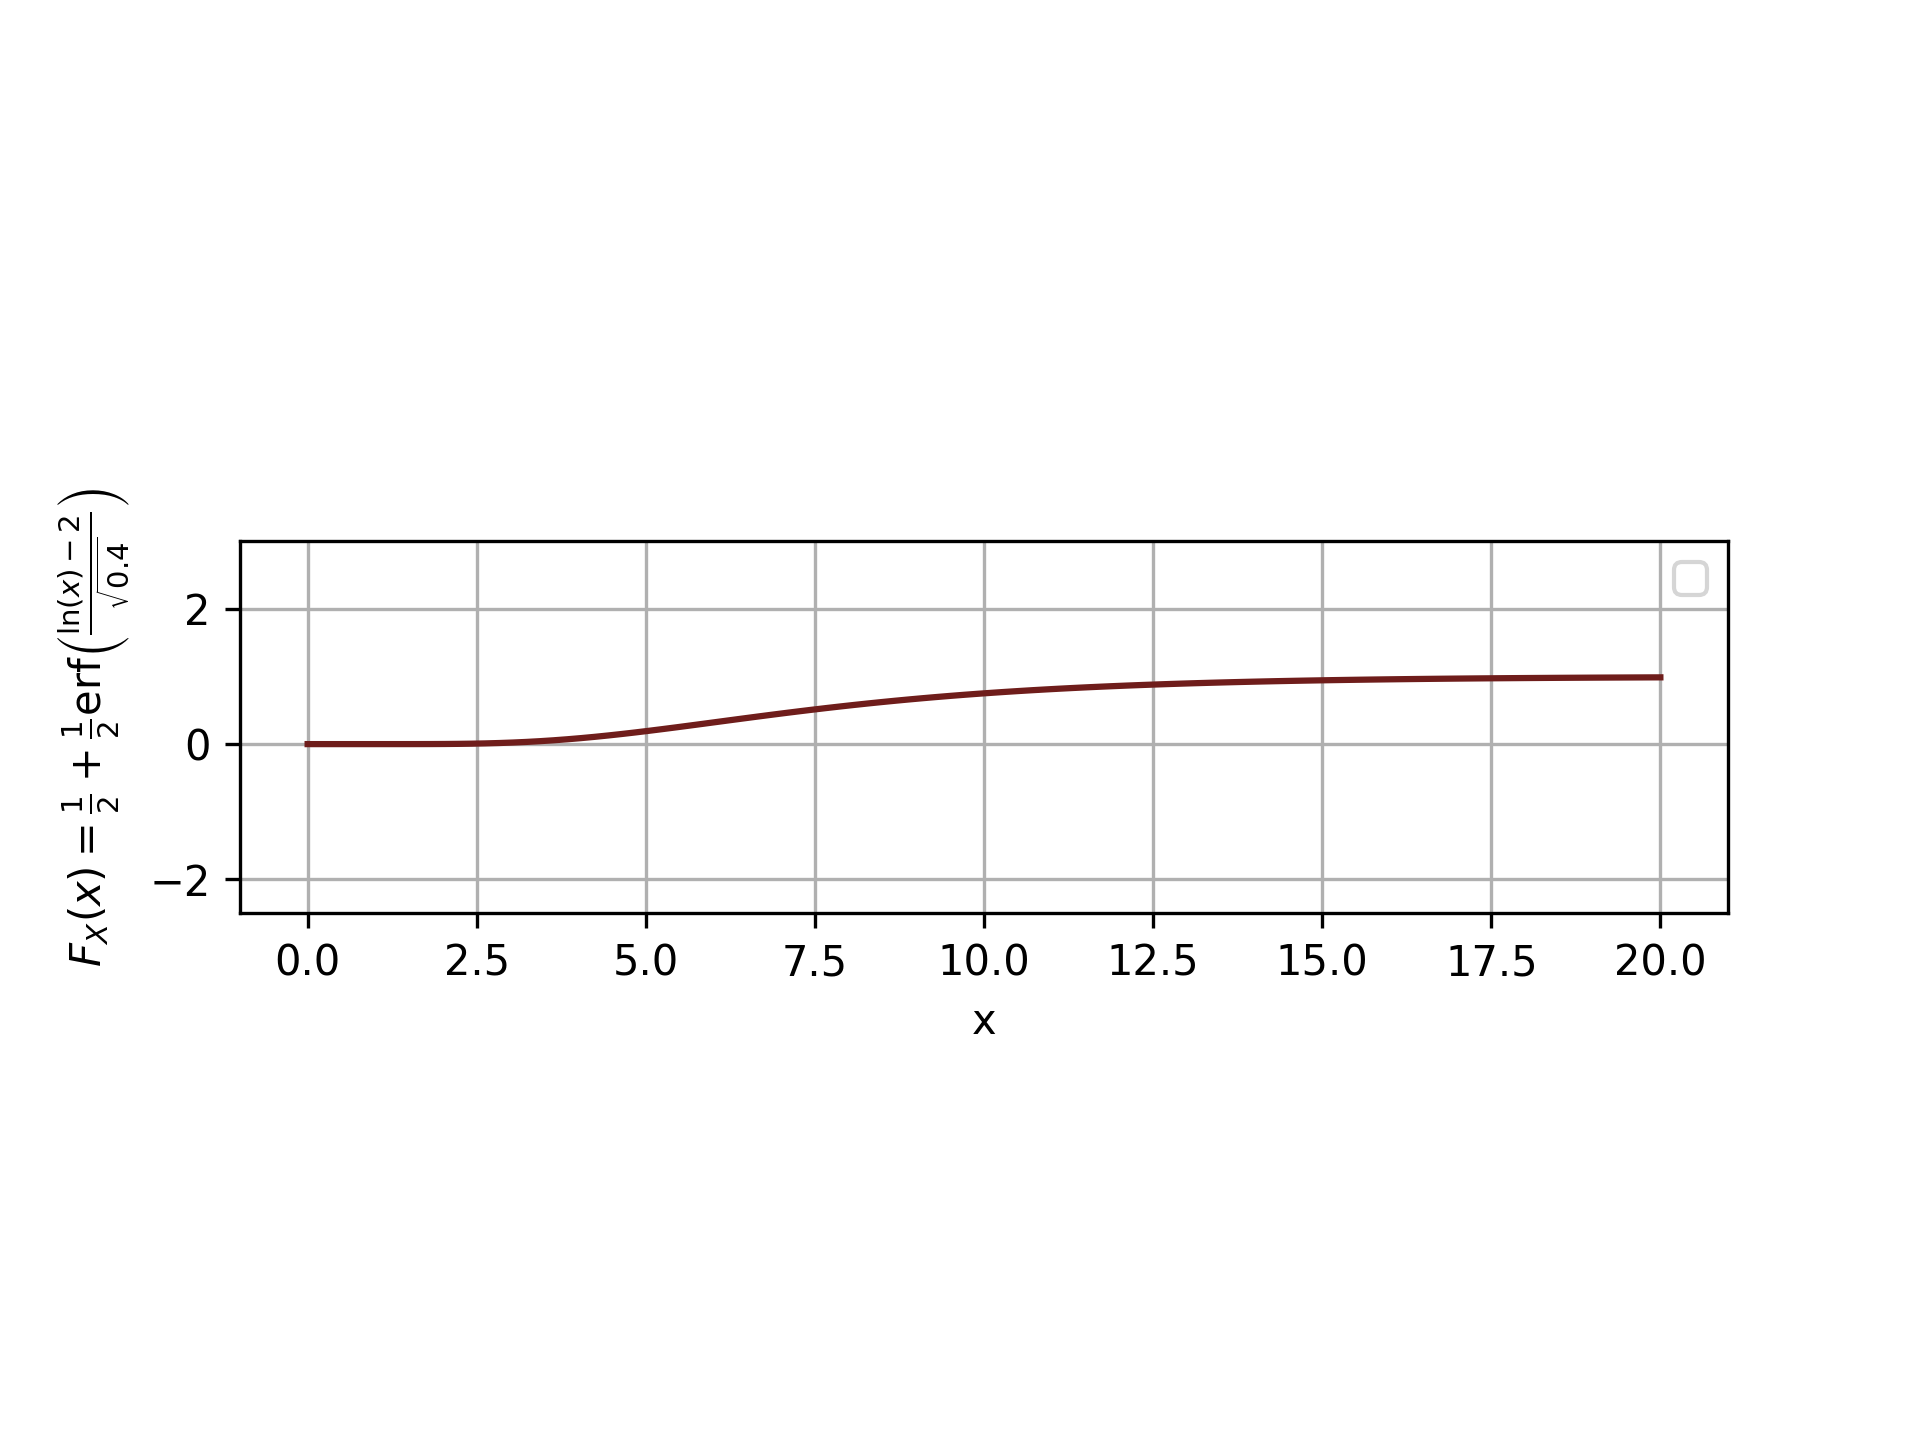
\includegraphics[width=1\textwidth]{cdf}
\vspace{-80pt}

Из графика видно, что функция (3) приблизительно принимает значения $0 < x < 20$ при $0 < y < 1$. 
Исходя из этого подберем вектор начальных приближений: \\ \null
[0, 3, 6, 9, 12, 15, 18, 21]. \\

Итого имеем:

\begin{lstlisting}[language=Python]
guesses = [0, 3, 6, 9, 12, 15, 18, 21]
for ind, el in enumerate(data):
    for attempt, guess in enumerate(guesses):
        try: 
            inv_value = inverse(el, guess)
            data[ind] = inv_value
            break
        except:
            pass

        if attempt == len(guesses) - 1:
            raise Exception('Solution was not found')
\end{lstlisting}

\noindent
\begin{adjustbox}{max width=1\textwidth}
  \parbox{\linewidth}{%
    \begin{gather*}
      X = [ \\
      \begin{aligned}
        & 7.129497868653516,  & \hspace{3pt} & 5.75990939608953,  & \hspace{3pt} & 10.709998315639028, & \hspace{3pt} & 6.344319895512703, & \\
        & 6.591160899999072,  & \hspace{3pt} & 3.784860187755976, & \hspace{3pt} & 6.977904630768007,  & \hspace{3pt} & 7.761423453312197, & \\
        & 6.932399313501684,  & \hspace{3pt} & 4.180285314129899, & \hspace{3pt} & 6.14211341489262,   & \hspace{3pt} & 3.6757503707970156,& \\ 
        & 10.753239775187453, & \hspace{3pt} & 6.671716126948868, & \hspace{3pt} & 14.643019921504544, & \hspace{3pt} & 8.572755366367943, & \\ 
      \end{aligned} \\
      ...\\
      ]
    \end{gather*}
  }
\end{adjustbox}

\subsection{Часть 2}\vspace{-20pt}\rule{\linewidth}{0.1mm}

Для полученной выборки найдите гистограмму относительных частот. 
Постройте на одном рисунке графики теоретической плотности $p(x)$ и 
гистограмму относительных частот.

\subsubsection{Первоначальная обработка полученных статистических данных}

\paragraph{Крайние члены вариационного ряда и размах выборки}\vspace{-20pt}\rule{\linewidth}{0.1mm}

Найдем крайние члены вариационного ряда как минимальное и максимальное значения 
набора данных, а также размах выборки, как их разницу:

\vspace{10pt}

\begin{lstlisting}[language=Python]
mini, maxi = min(data), max(data)
print(mini, maxi)

range_ = maxi - mini
print(range_)
\end{lstlisting}

\vspace{-5pt}

\begin{align*}
  & \text{Крайние члены: }  3.1658, \hspace{5pt} 36.3487 \\
  & \text{Размах выборки: }  33.1829
\end{align*}

{\footnotesize \textbf{Примечание:} Выводимые данные округлены до 4х знаков для удобства чтения.}

\newpage

\paragraph{Группировка данных}\vspace{-20pt}\rule{\linewidth}{0.1mm}

Для начала определим количество интервалов, воспользовавшись правилом
Стерджеса:
\begin{equation*}
    k = 1 + \lfloor \log_2 n \rfloor,
\end{equation*}
где $n$ — общее число наблюдений величины, \\ 
$\log_2$ — логарифм по основанию 2, \\
$\lfloor x \rfloor$ — обозначает целую часть числа $x$. \\

И определим шаг интервала разделив размах выборки на количество интервалов:

\vspace{10pt}

\begin{lstlisting}[language=Python]
trunc = lambda x : int(str(x)[:str(x).index('.')])
k = 1 + trunc(np.log2(n))
h = range_ / k
\end{lstlisting}

\vspace{-5pt}

\begin{align*}
    & \text{Количество интервалов: } 7 \\
    & \text{Шаг интервала: }  4.7404
\end{align*}

Теперь сгруппируем данные:

\vspace{10pt}

\begin{lstlisting}[language=Python]
grouped_data = []

begin = mini
for i in range(k):
    end = begin + h

    middle = (begin + end) / 2
    freq = sum(begin <= el < end for el in data)
    
    if i == k - 1:
        freq += 1

    relative_freq = freq / n

    grouped_element = {
        'interval numero': i,
        'interval': f'[{begin}, {end})',
        'middle': middle,
        'frequency': freq,
        'relative frequency': relative_freq
    }
    grouped_data.append(grouped_element)

    begin = end
\end{lstlisting}
\vspace{10pt}
Полученную группировку представим в виде таблицы:
\vspace{10pt}
\begin{table}[h!]
  \centering
  \renewcommand{\arraystretch}{1.5}
  \begin{adjustbox}{max width=0.8\textwidth}
      \begin{tabular}{|c|c|c|c|c|c|}
      \hline
      номер     & \multirow{2}{*}{интервал} & середина  & \multirow{2}{*}{частота} & относительная \\
      интервала &                           & интервала &                          & частота       \\
      \hline
      0 & [3.1658,  7.9062)  & 5.5360  & 69 & 0.575 \\ 
      \hline
      1 & [7.9062,  12.6466) & 10.2764 & 36 & 0.3 \\ 
      \hline
      2 & [12.6466, 17.3870) & 15.0168 & 10 & 0.08333 \\ 
      \hline
      3 & [17.3870, 22.1274) & 19.7572 & 3  & 0.025 \\ 
      \hline
      4 & [22.1274, 26.8679) & 24.4977 & 1  & 0.00833 \\ 
      \hline
      5 & [26.8679, 31.6083) & 29.2381 & 0  & 0.0 \\ 
      \hline
      6 & [31.6083, 36.3487) & 33.9785 & 1  & 0.00833 \\ 
      \hline
      \end{tabular}
  \end{adjustbox}
  \caption{Сгруппированные данные}
  \label{tab:your_table_label}
\end{table}

% ------------------------------------LITERATURE------------------------------------

\newpage
\section{Список использованных источников}\vspace{-20pt}\rule{\linewidth}{0.1mm}
\begin{enumerate}
  \item \label{item:source1} L'Ecuyer, Pierre (January 1999). "Tables of Linear Congruential Generators of Different Sizes and Good Lattice Structure" - С. 256
\end{enumerate}

\end{document}
